% !TEX root = ../main.tex
\subsubsection{Statistics Study}
\label{14.32::statistics_study}
    After obtaining the $v_z$ region with the maximum range of kinematic variables, our second criterion is to maximise statistics inside this region.
    With phase space already maximised, this allows us to increase the statistical precision of future studies, enabling a thorough exploration of the parameter space.

    Based on the results of the different phase space studies, we'll limit the scope of this statistics study to the region $-5 \text{cm} < v_z < 10 \text{cm}$, the result of which can be observed in Figure \ref{fig::14.32::statistics}.
    The objective of this study is to find the 7 cm region in $v_z$ with the highest statistics.
    The choice of 7 cm in particular comes from the length of the double target, where the liquid target has a length of 3 cm, the separation between the liquid and solid target is 4 cm, and the solid target is of negligible width for the scope of this study.

    First, we look at $e^-$ statistics, seen in Figure \ref{fig::14.32::statistics_11}.
    It is trivial to note that, in the studied range, the more upstream we look, the more statistics are seen.
    Therefore, the best region for the placement of the target is from $-5$ to $2$ cm.
    This result is only reinforced by the results observed in $e^-\pi^+$ and $e^-\pi^-$ statistics, which can be seen in Figures \ref{fig::14.32::statistics_211} and \ref{fig::14.32::statistics_-211}.

    % statistics.
    \begin{figure}
        \centering
        % e-.
        \begin{subfigure}[b]{\textwidth}
            \centering
            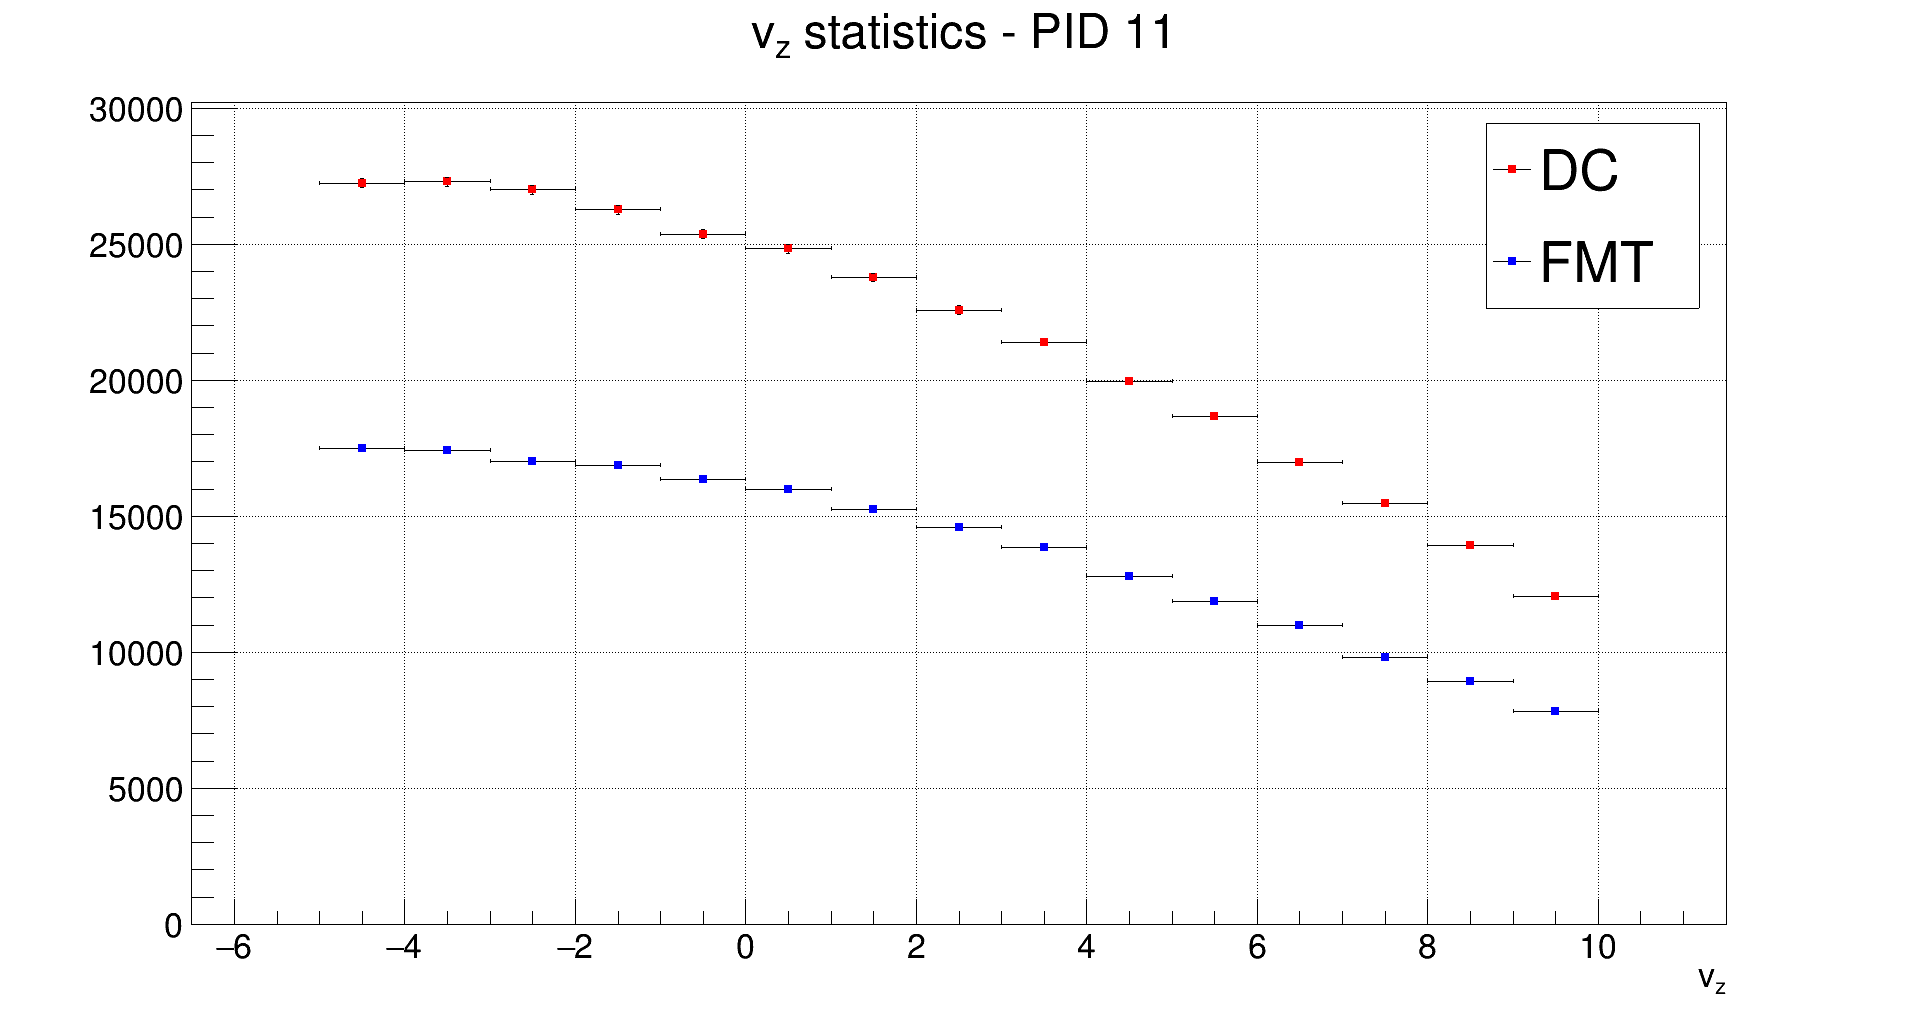
\includegraphics[width=\textwidth]{32statistics_11.png}
            \caption{$e^-$ statistics.}
            \label{fig::14.32::statistics_11}
        \end{subfigure}
        \centering
        % e-pi+.
        \begin{subfigure}[b]{0.49\textwidth}
            \centering
            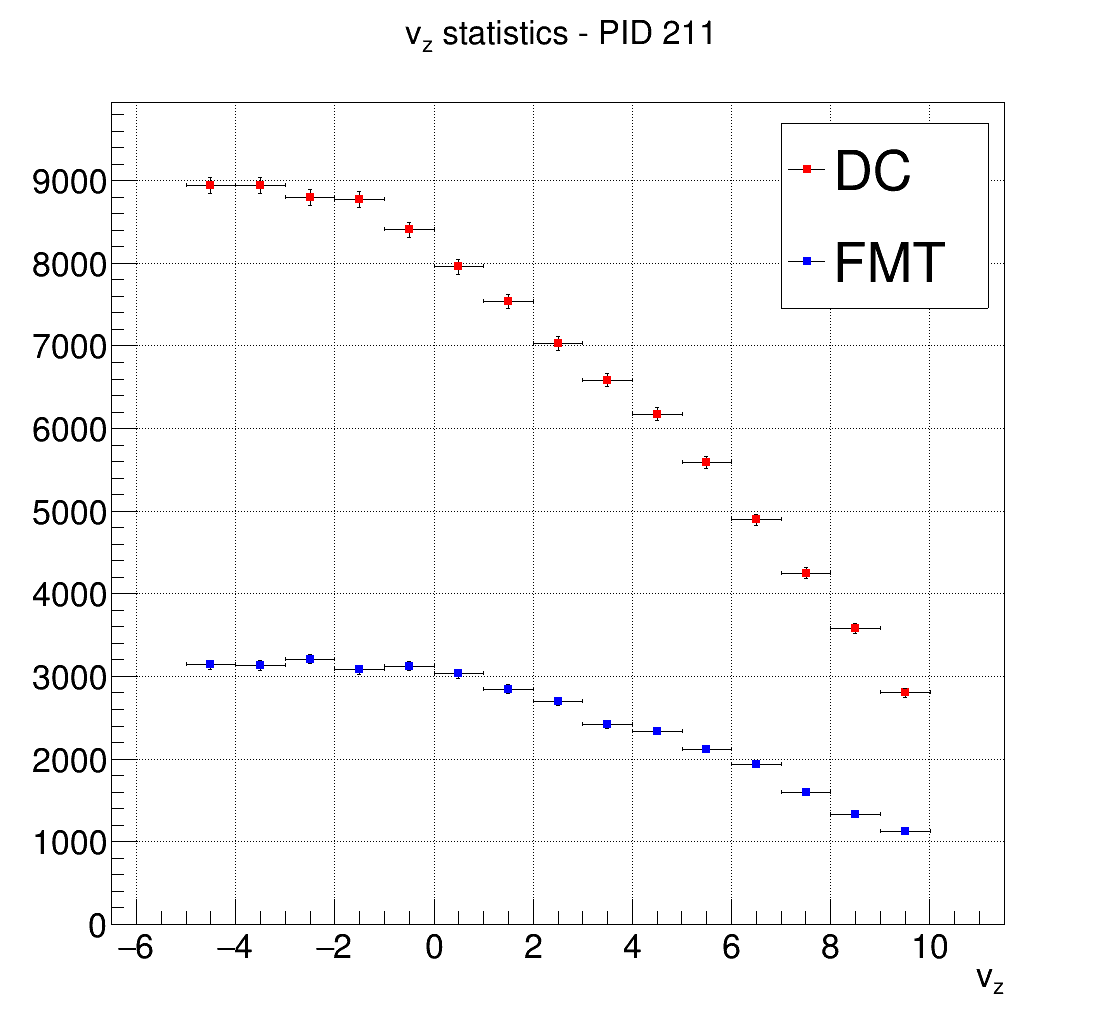
\includegraphics[width=\textwidth]{32statistics_211.png}
            \caption{$e^-\pi^+$ statistics.}
            \label{fig::14.32::statistics_211}
        \end{subfigure}
        \hfill
        % e-pi-.
        \begin{subfigure}[b]{0.49\textwidth}
            \centering
            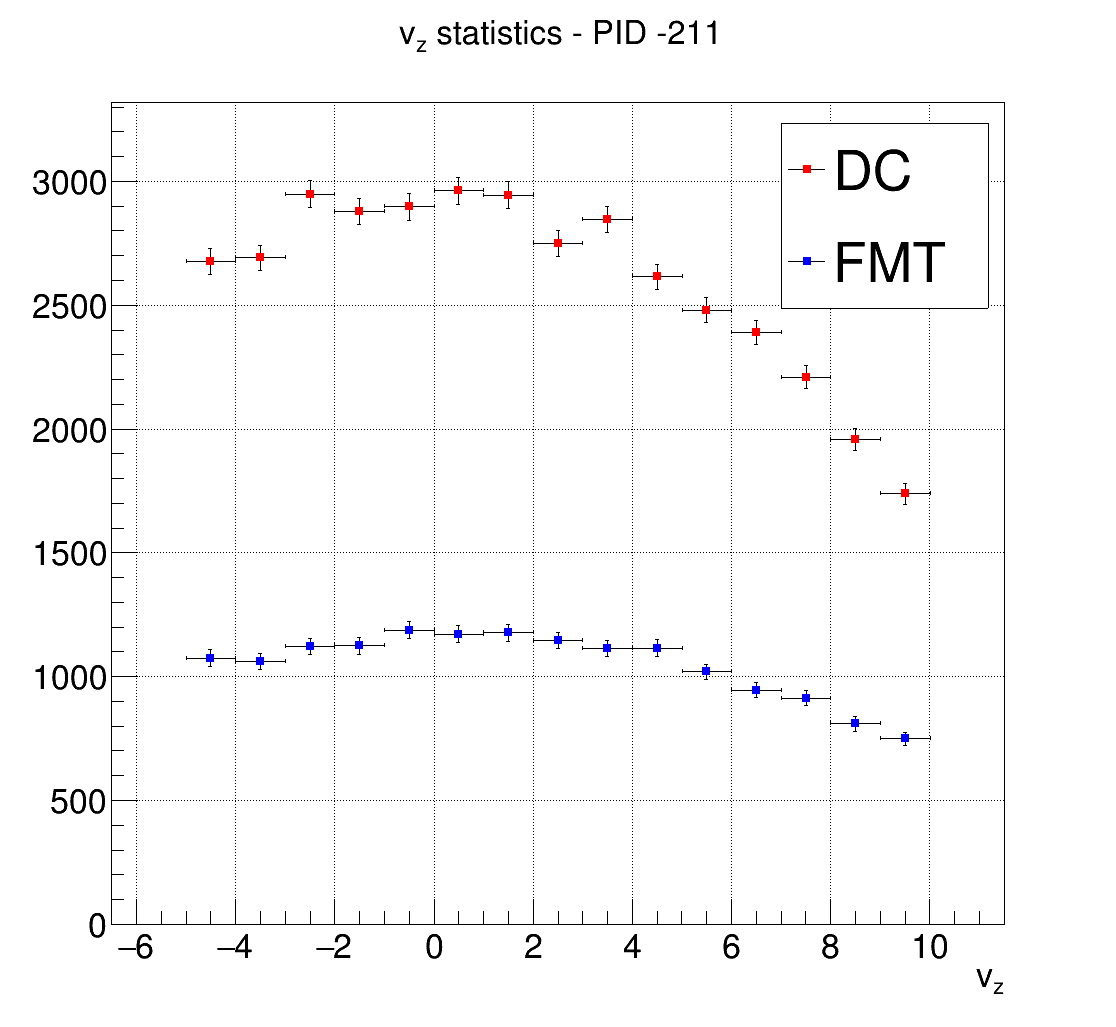
\includegraphics[width=\textwidth]{32statistics_-211.png}
            \caption{$e^-\pi^-$ statistics.}
            \label{fig::14.32::statistics_-211}
        \end{subfigure}
        \caption[Statistics for $e^-$, $e^-\pi^+$, and $e^-\pi^-$ against $v_z$]
        {$e^-$, $e^-\pi^+$, and $e^-\pi^-$ statistics against $v_z$ for run 12016.
        No acceptance correction was applied to these results.}
        \floatfoot{Source: Own elaboration, using the \href{https://github.com/bleaktwig/clas12-rge-analysis}{clas12-rge-analysis} software.}
        \label{fig::14.32::statistics}
    \end{figure}
